\section{Introduction}
Deep learning methods have been successful in a broad spectrum of real-world tasks, including computer vision~\cite{godard2017unsupervised,he2016deep}, natural language processing~\cite{zhao2023evaluating,devlin2018bert,vaswani2017attention}, and medical domain~\cite{ye2023bidirectional}. %In these contexts, the assessment of model uncertainty emerges as a vital component. Uncertainty within the context of deep learning can typically be classified into two principal categories: the irreducible inherent randomness of data, the \textit{aleatoric uncertainty}, and the uncertainty related to model parameters, the \textit{epistemic uncertainty}~\cite{gal2016dropout,guo2017calibration}.
In these scenarios, evaluating model uncertainty becomes a crucial element. Within the realm of deep learning, uncertainty is generally categorized into two primary groups: the intrinsic randomness inherent in data, referred to as the \textit{aleatoric uncertainty}, and the uncertainty associated with model parameters, known as the \textit{epistemic uncertainty}~\cite{gal2016dropout,guo2017calibration}.

%Among these, the representation of epistemic uncertainty presents a particular challenge, owing to the inherent difficulty associated with accurately quantifying the uncertainty tied to the model's parameters. 
Among these, accurately quantifying the uncertainty linked to the model's parameters proves to be a particularly demanding task, due to the inherent complexity involved.
To tackle this, strategies such as Ensemble-based methods~\cite{pearce2020uncertainty,lakshminarayanan2017simple} and Bayesian neural networks (BNNs)~\cite{gal2016dropout,wilson2020bayesian,blundell2015weight} have been proposed to measure epistemic uncertainty. 
%However, they either require extensive computational cost or have scalability issues. To solve these issues, evidential deep learning methods~\cite{sensoy2018evidential,NEURIPS2020_aab08546,malinin2018predictive} have been conceived, designed to address uncertainty estimation by generating parameters of distributions as its outputs.
Nonetheless, these methods either demand substantial computational resources or encounter challenges in scalability. In response to these limitations, the concept of evidential deep learning techniques~\cite{sensoy2018evidential,NEURIPS2020_aab08546,malinin2018predictive} has emerged. These methods are formulated to handle uncertainty estimation by producing distribution parameters as their output.



% instrumental in both the evaluation of model performance and the interpretation of prediction confidence. 
% Addressing this necessity, evidential deep learning methods have been conceived, specifically targeting the estimation of uncertainty.



\begin{figure}
  \centering
  \begin{tabular}{c}
       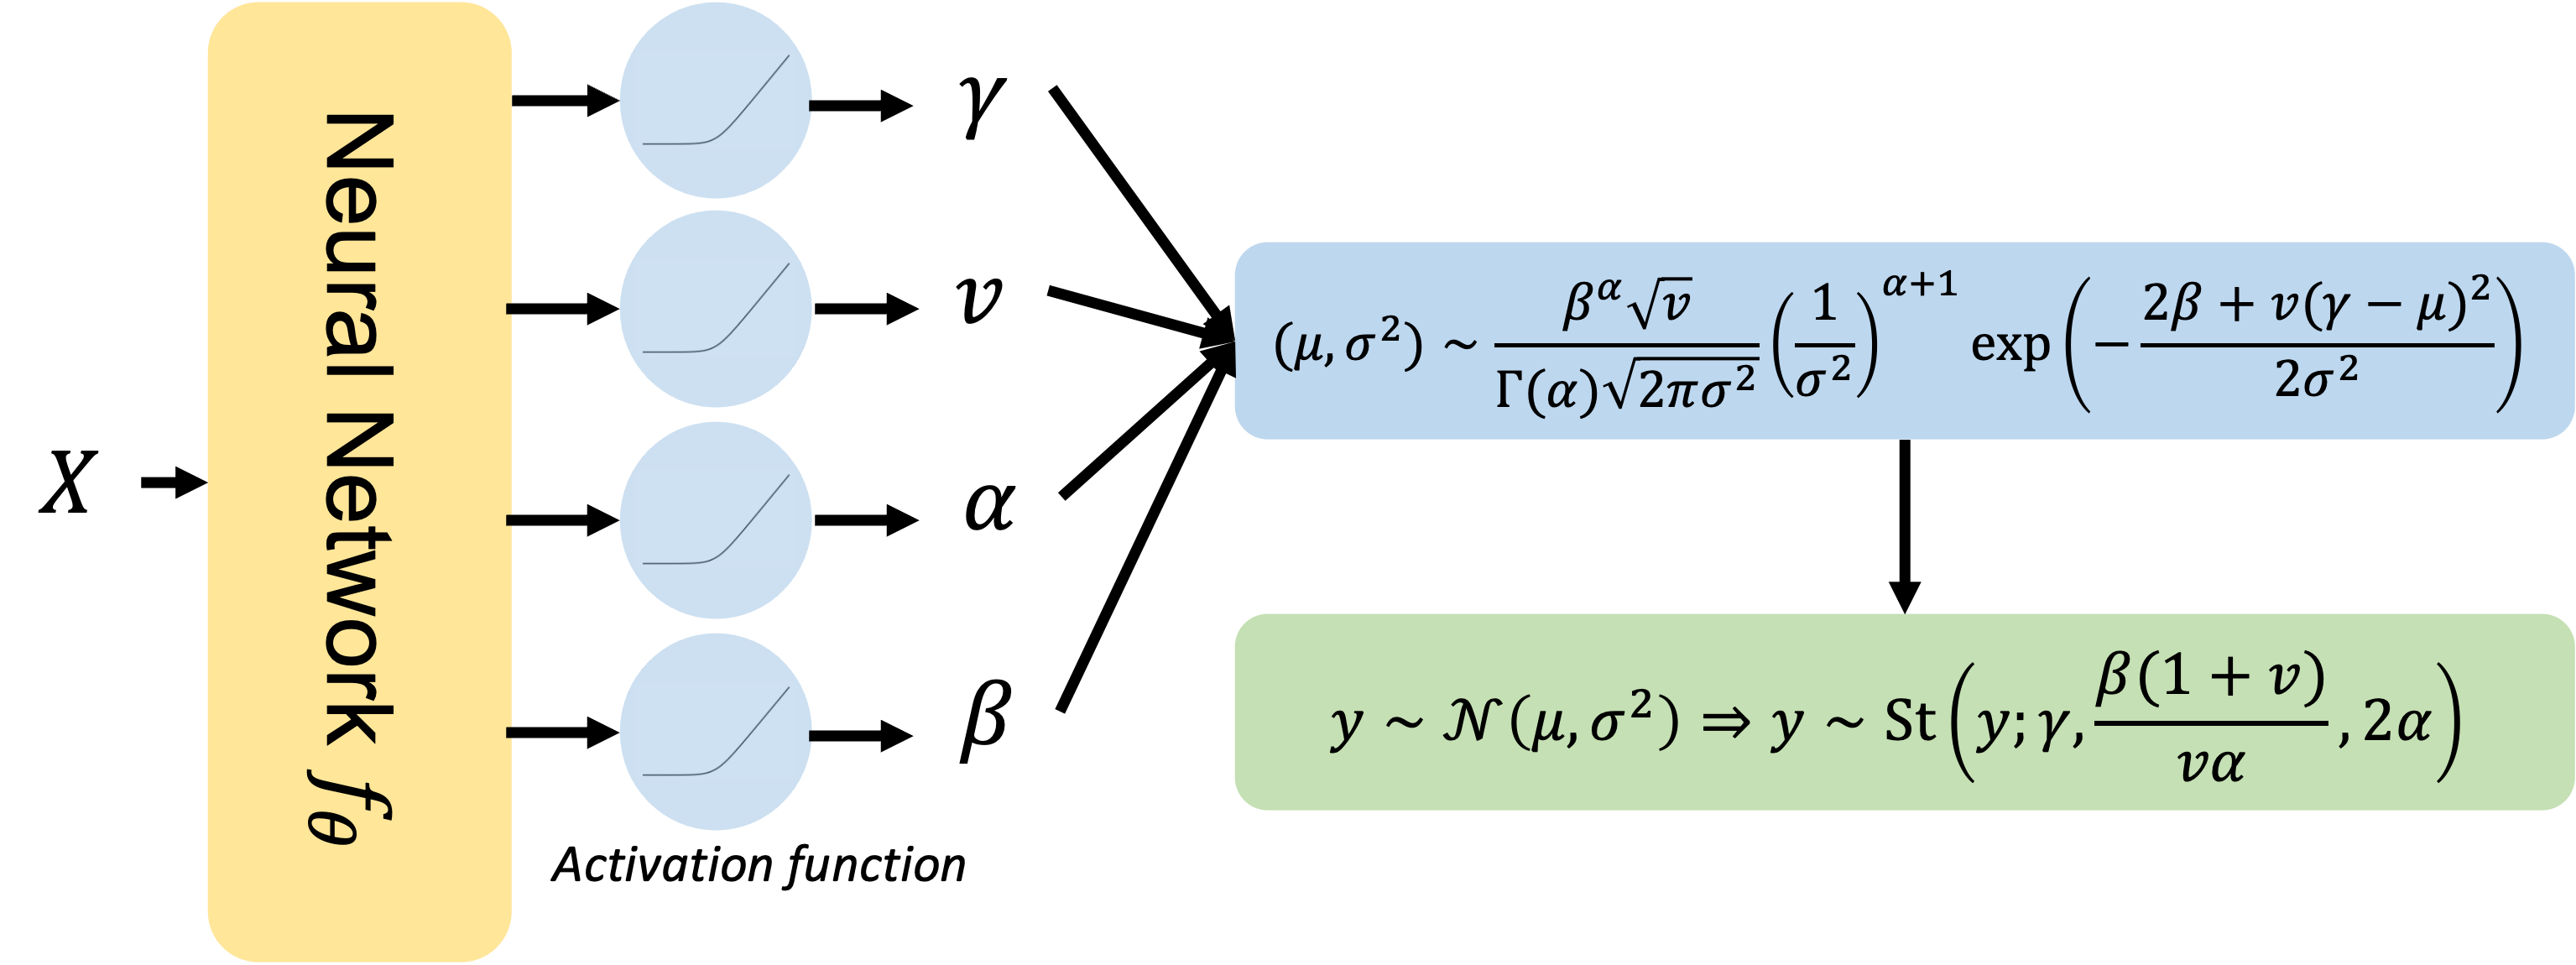
\includegraphics[width=0.9\linewidth]{nig_framework.png}  \\
       (a) Evidential Regression Network (ERN) architecture \\
       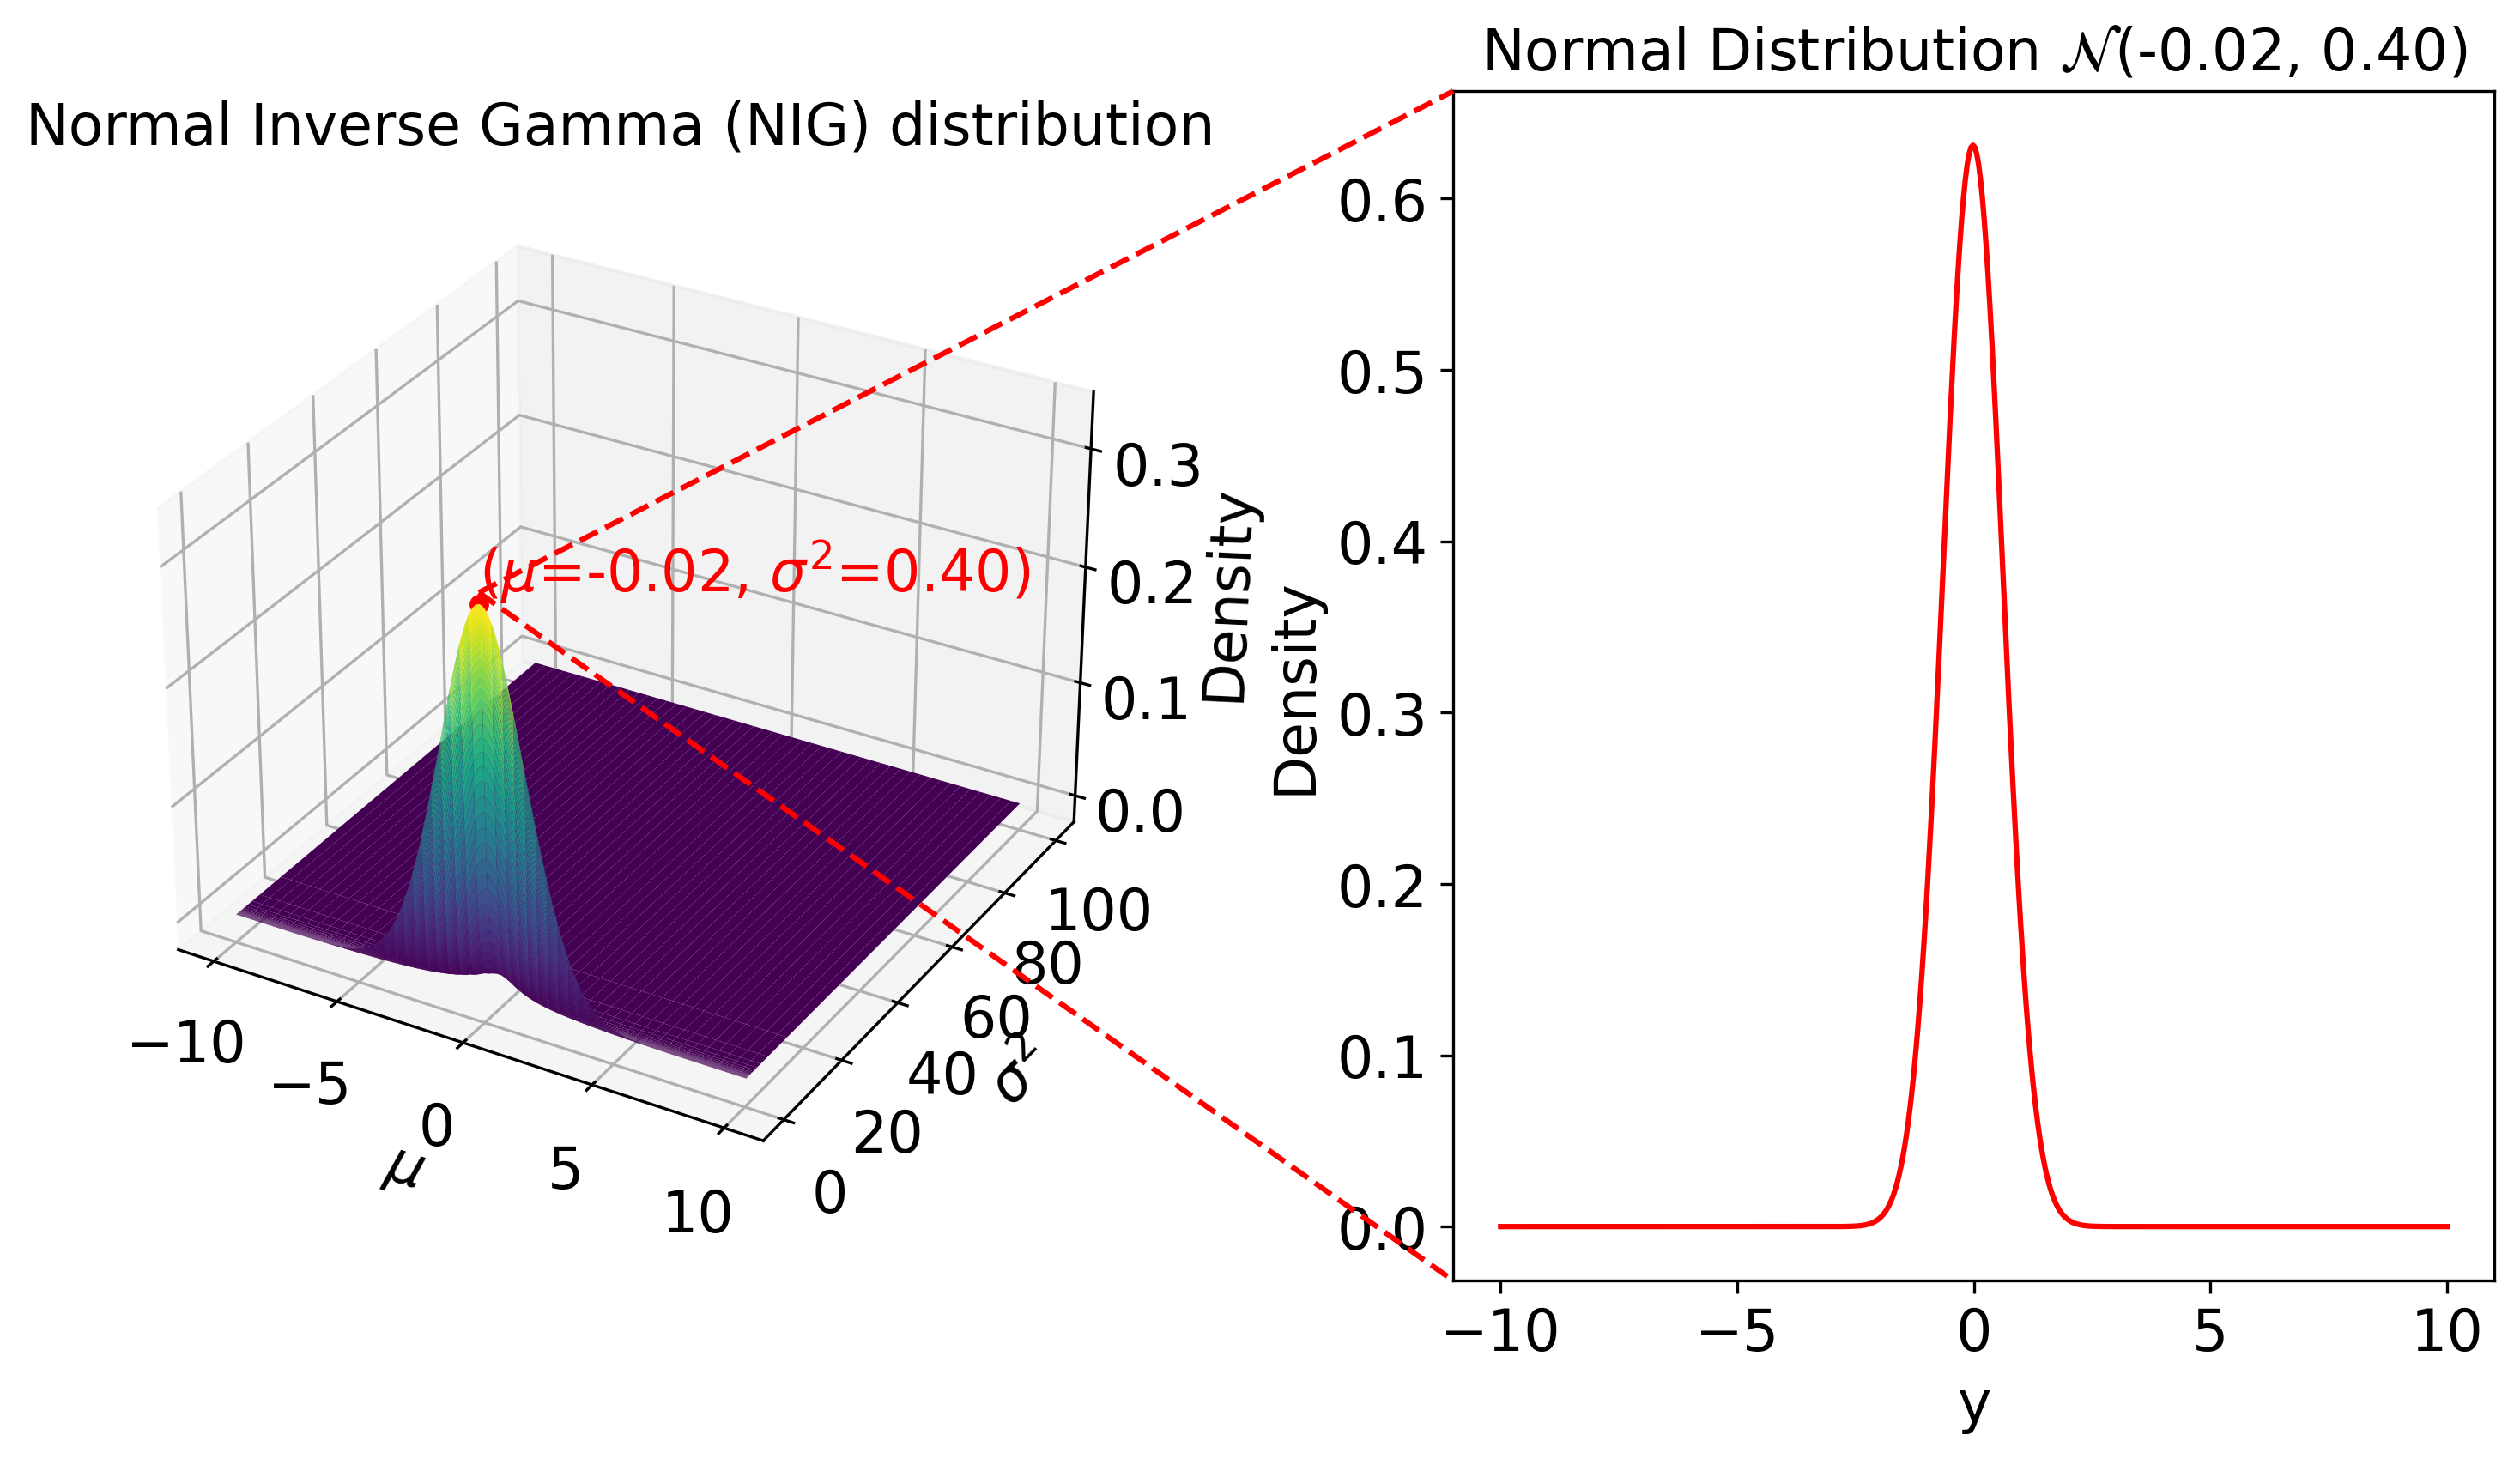
\includegraphics[width=0.9\linewidth]{nig_distribution.png}  \\
       (b) Normal Inverse-Gamma (NIG) distribution.\\
  \end{tabular}
  \caption{ An overview of the Evidential Regression Network (ERN) architecture with illustrations on the final distributions of the prediction. ERN outputs four predictions as distribution parameters, with activation functions like Relu or Softplus to constrain the output to meet the requirements of distribution parameters.}
  \label{uncertainty_framework}
\end{figure}


The Evidential Regression Network (ERN)~\cite{NEURIPS2020_aab08546} introduces a novel deep-learning regression approach that incorporates Dempster-Shafer theory~\cite{shafer1976mathematical} to quantify model uncertainty, resulting in impressive achievements. Within the ERN framework, the training process is conceptualized as an evidence acquisition process, which is inspired by evidential models for classification~\cite{malinin2018predictive,malinin2019reverse,bilovs2019uncertainty,haussmann2019bayesian,malinin2019ensemble}. 
During the training phase, ERN establishes prior distributions over the likelihood function, and each training sample contributes to the formation of a higher-order evidential distribution from which the likelihood function is drawn. 
During the inference phase, ERN produces the hyperparameters of the evidential distribution, facilitating both prediction and uncertainty estimation without the necessity for sampling. 
This approach was subsequently extended to multivariate regression tasks by~\citeauthor{meinert2021multivariate} using different prior distributions. 

Previous ERN methods \cite{NEURIPS2020_aab08546,malinin2020regression,charpentier2021natural,oh2022improving,feng2023deep,mei2023uncertainty} use specific activation functions like ReLU to ensure non-negative values for parameters of the evidential distribution, such as the variance.
Nevertheless, the utilization of such activation functions may inadvertently hinder ERN models' capacity to learn effectively from training samples, thereby impairing overall model performance~\cite{pandey2023learn}. 
%In classification, evidential models have shown suboptimal results because of `zero confidence regions' within the evidential space
%In classification, evidential models have demonstrated suboptimal results due to the presence of `zero confidence regions` within the evidential space~\cite{pandey2023learn}. 
Furthermore, in classification tasks, evidential models have underperformed because of the existence of "zero confidence regions" within the evidential space~\cite{pandey2023learn}.

%However, analysis for evidential models in the context of regression tasks is notably lacking.

However, there is a notable lack of convergence analysis for evidential models in the context of regression tasks.
In this paper, we explore the existence of zero confidence regions, which result in high uncertainty areas (HUA) during the training process of ERN models for regression tasks.
Building upon the insights derived from our analysis, we propose a novel regularization term that enables the ERN to bypass the HUA and effectively learn from the zero-confidence regions. 
We also show that the proposed regularization can be generalized to various ERN variants.
We conduct experiments on both synthetic and real-world data and show the effectiveness of the proposed method\footnote{Code is at https://github.com/FlynnYe/UR-ERN}. 
The main contributions of our work are summarized as follows:
\begin{itemize}
\item We revealed the existence of HUA in the learning process of ERN methods with theoretical analysis. The existence of HUA impedes the learning ability of evidential regression models, particularly in regions where ERN exhibits low confidence.
\item We propose a novel uncertainty regularization term designed to handle this HUA in evidential regression models and provide theoretical proof of its effectiveness.
\item Extensive experiments across multiple datasets and tasks are conducted to validate our theoretical findings and demonstrate the effectiveness of our proposed solution.
\end{itemize}





% Deep learning methods have been successful in a broad spectrum of real-world tasks, including computer vision~\cite{godard2017unsupervised,he2016deep}, natural language processing~\cite{zhao2023evaluating,devlin2018bert,vaswani2017attention}, and speech recognition~\cite{kamath2019deep}. %In these contexts, the assessment of model uncertainty emerges as a vital component. Uncertainty within the context of deep learning can typically be classified into two principal categories: the irreducible inherent randomness of data, the \textit{aleatoric uncertainty}, and the uncertainty related to model parameters, the \textit{epistemic uncertainty}~\cite{gal2016dropout,guo2017calibration}.
% In these scenarios, evaluating model uncertainty becomes a crucial element. Within the realm of deep learning, uncertainty is generally categorized into two primary groups: the intrinsic randomness inherent in data, referred to as the \textit{aleatoric uncertainty}, and the uncertainty associated with model parameters, known as the \textit{epistemic uncertainty}~\cite{gal2016dropout,guo2017calibration}.

% %Among these, the representation of epistemic uncertainty presents a particular challenge, owing to the inherent difficulty associated with accurately quantifying the uncertainty tied to the model's parameters. 
% Among these, accurately quantifying the uncertainty linked to the model's parameters proves to be a particularly demanding task, due to the inherent complexity involved.
% To tackle this, strategies such as Ensemble-based methods~\cite{pearce2020uncertainty,lakshminarayanan2017simple} and Bayesian neural networks (BNNs)~\cite{gal2016dropout,wilson2020bayesian,blundell2015weight} have been proposed to measure epistemic uncertainty. 
% %However, they either require extensive computational cost or have scalability issues. To solve these issues, evidential deep learning methods~\cite{sensoy2018evidential,NEURIPS2020_aab08546,malinin2018predictive} have been conceived, designed to address uncertainty estimation by generating parameters of distributions as its outputs.
% Nonetheless, these methods either demand substantial computational resources or encounter challenges in scalability. In response to these limitations, the concept of evidential deep learning techniques~\cite{sensoy2018evidential,NEURIPS2020_aab08546,malinin2018predictive} has emerged. These methods are formulated to handle uncertainty estimation by producing distribution parameters as their output.



% % instrumental in both the evaluation of model performance and the interpretation of prediction confidence. 
% % Addressing this necessity, evidential deep learning methods have been conceived, specifically targeting the estimation of uncertainty.



% \begin{figure}
%   \centering
%   \begin{tabular}{c}
%        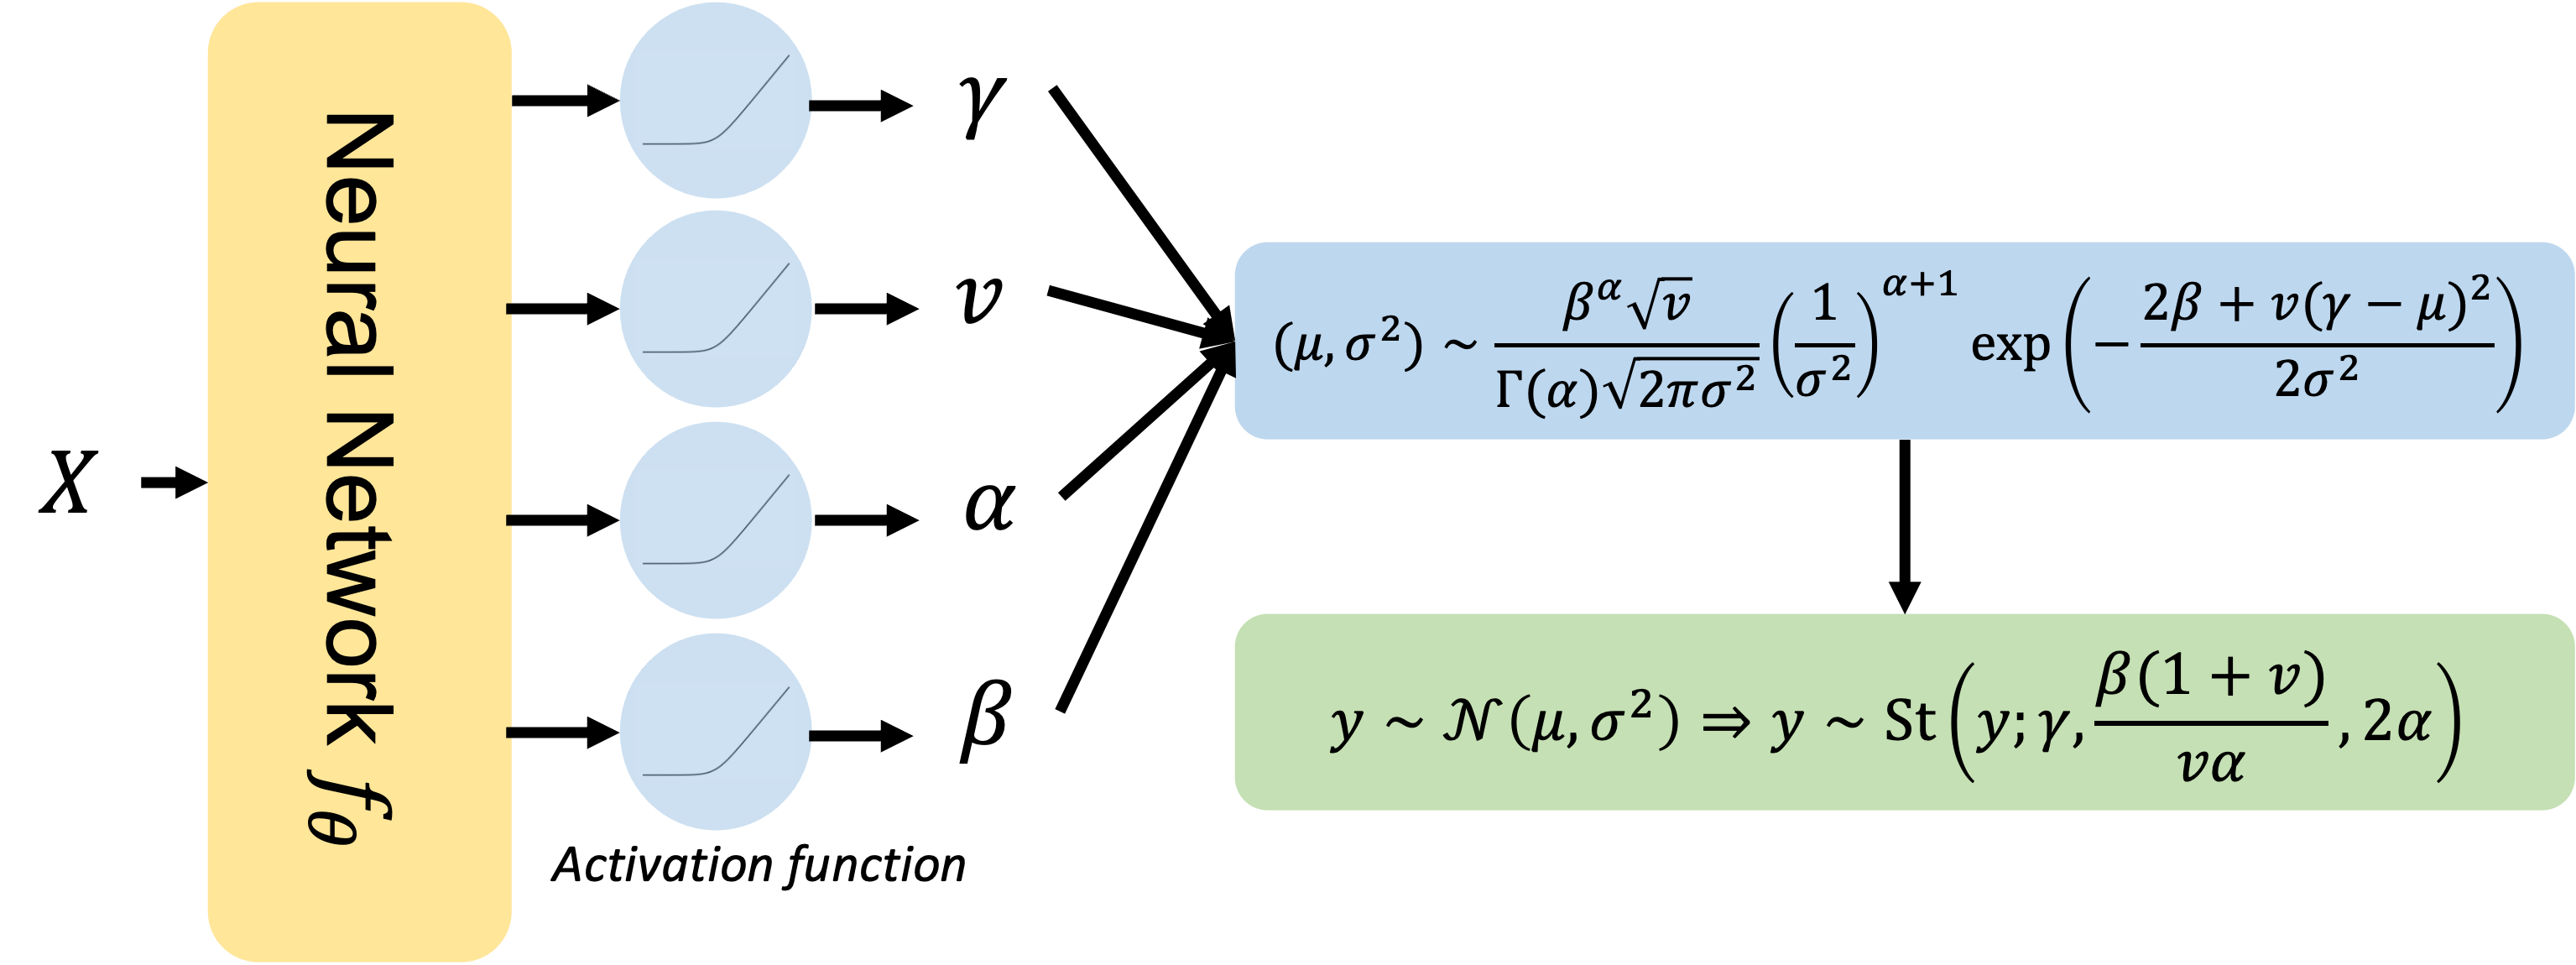
\includegraphics[width=0.9\linewidth]{nig_framework.png}  \\
%        (a) Evidential Regression Network (ERN) architecture \\
%        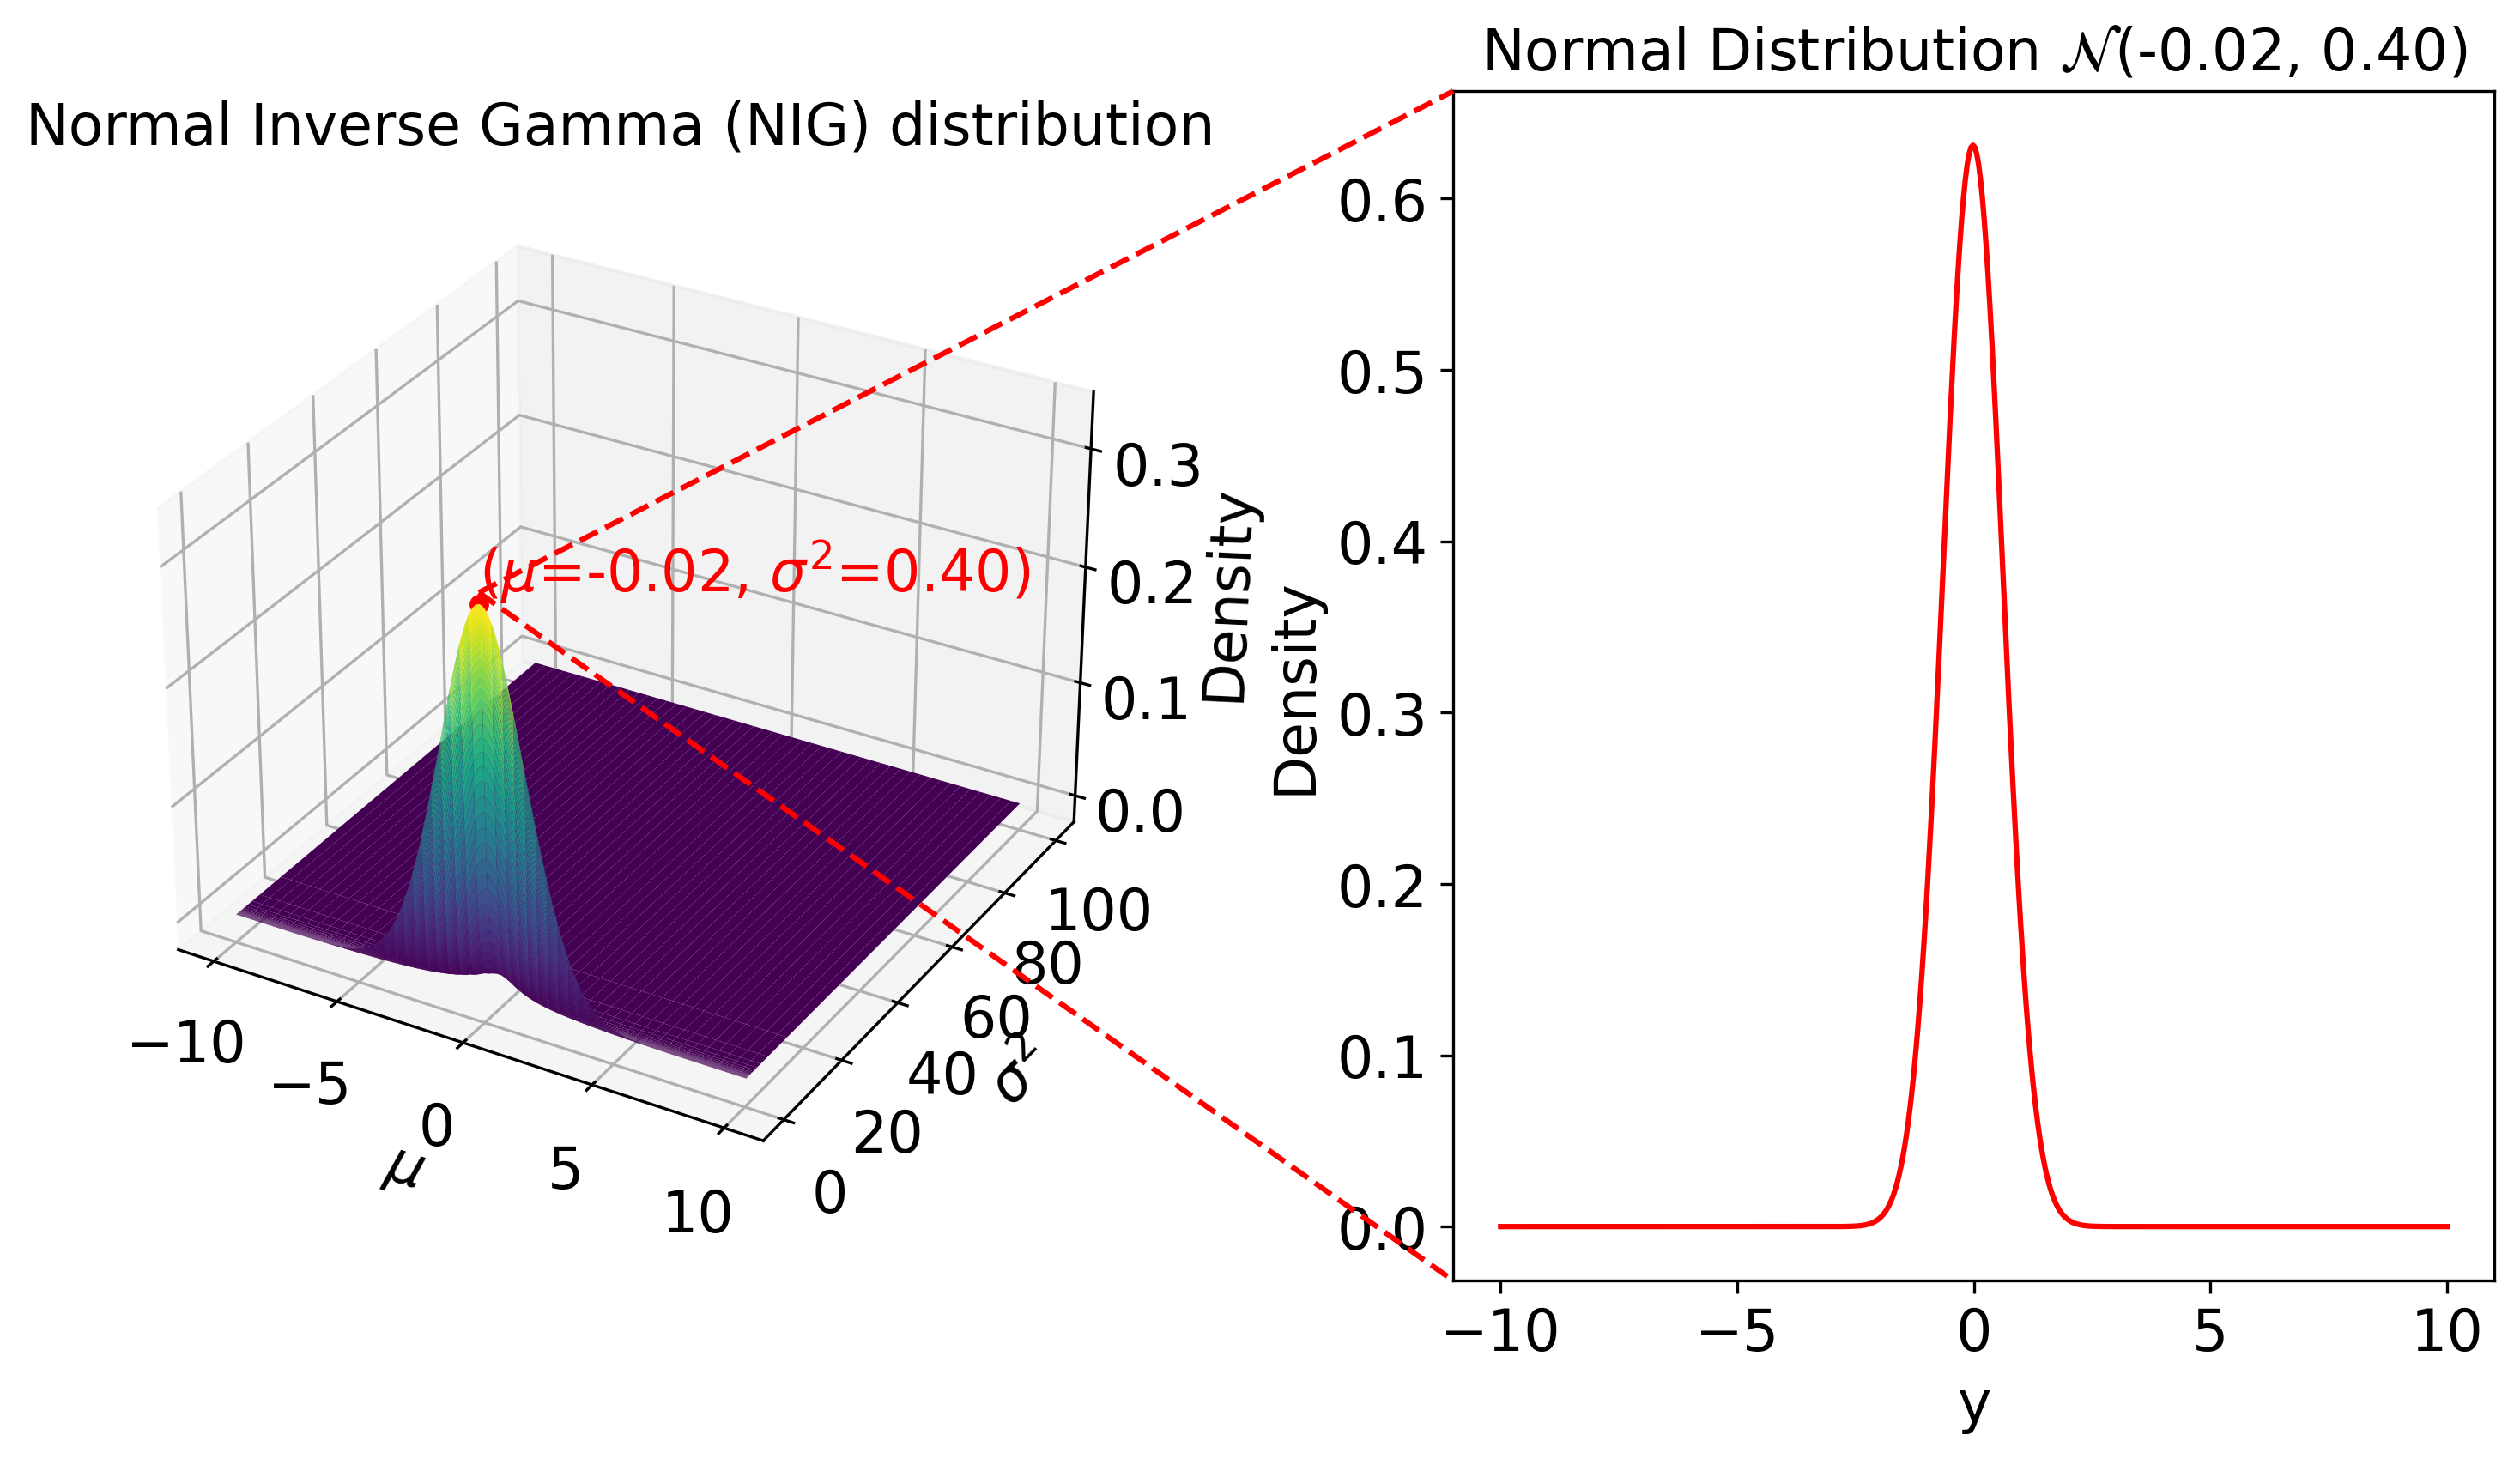
\includegraphics[width=0.9\linewidth]{nig_distribution.png}  \\
%        (b) Normal Inverse-Gamma (NIG) distribution.\\
%   \end{tabular}
%   \caption{ An overview of the Evidential Regression Network (ERN) architecture with illustrations on the final distributions of the prediction. ERN outputs four predictions as distribution parameters, with activation functions like Relu or Softplus to constrain the output to meet the requirements of distribution parameters.}
%   \label{uncertainty_framework}
% \end{figure}


% The Evidential Regression Network (ERN)~\cite{NEURIPS2020_aab08546} introduces a novel deep-learning regression approach that incorporates Dempster-Shafer theory~\cite{shafer1976mathematical} to quantify model uncertainty, resulting in impressive achievements. Within the ERN framework, the training process is conceptualized as an evidence acquisition process, which is inspired by evidential models for classification~\cite{malinin2018predictive,malinin2019reverse,bilovs2019uncertainty,haussmann2019bayesian,malinin2019ensemble}. 
% During the training phase, ERN establishes prior distributions over the likelihood function, and each training sample contributes to the formation of a higher-order evidential distribution from which the likelihood function is drawn. 
% During the inference phase, ERN produces the hyperparameters of the evidential distribution, facilitating both prediction and uncertainty estimation without the necessity for sampling. 
% This approach was subsequently extended to multivariate regression tasks by~\citeauthor{meinert2021multivariate} using different prior distributions. 

% Previous ERN methods \cite{NEURIPS2020_aab08546,malinin2020regression,charpentier2021natural,oh2022improving} use specific activation functions like ReLU to ensure non-negative values for parameters of the evidential distribution, such as the variance.
% Nevertheless, the utilization of such activation functions may inadvertently hinder ERN models' capacity to learn effectively from training samples, thereby impairing overall model performance~\cite{pandey2023learn}. 
% %In classification, evidential models have shown suboptimal results because of `zero confidence regions' within the evidential space
% %In classification, evidential models have demonstrated suboptimal results due to the presence of `zero confidence regions` within the evidential space~\cite{pandey2023learn}. 
% Furthermore, in classification tasks, evidential models have underperformed because of the existence of "zero confidence regions" within the evidential space~\cite{pandey2023learn}.

% %However, analysis for evidential models in the context of regression tasks is notably lacking.

% However, there is a notable lack of analysis for evidential models in the context of regression tasks, let alone the 'zero confidence regions' issue.
% In this paper, we explore the widespread presence of zero confidence regions, which result in areas of high uncertainty (HUA) during the learning process of ERN models for regression tasks.
% Building upon the insights derived from our analysis, we propose a novel regularization term that enables the ERN to bypass the HUA and effectively learn from the zero-confidence regions. 
% We also show that the proposed regularization can be generalized to various ERN variants.
% We conduct experiments on both synthetic and real-world data and showcase the effectiveness of the proposed method. 
% The main contributions of our work are summarized as follows:
% \begin{itemize}
% \item We revealed the existence of HUA in the learning process of ERN methods with theoretical analysis. The existence of HUA impedes the learning ability of evidential regression models, particularly in regions where ERN exhibits low confidence.
% \item We propose a novel uncertainty regularization term designed to handle this HUA in evidential regression models and provide theoretical proof of its effectiveness.
% \item Extensive experiments across multiple datasets and tasks are conducted to validate our theoretical findings and demonstrate the effectiveness of our proposed solution.
% \end{itemize}


